\selectlanguage{italian}
\section{Definizioni e nomenclatura}

Un nuclide (o nucleo) è una specifica combinazione di protoni e neutroni: si definiscono il numero atomico $ Z $ come il numero di protoni, il numero di neutroni $ N $ ed il numero di massa $ A = Z + N $ come il numero di nucleoni. In un atomo neutro, $ Z $ è anche il numero totale di elettroni negli orbitali.\\
Il simbolo completo di un nuclide è $ ^A_Z \text{X}_N $, dove $ \text{X} $ è il simbolo della specie chimica: tale scrittura è però ridondante, poiché la specie chimica definisce di per sé il numero di protoni nel nuclide, dunque è sufficiente scrivere $ ^A \text{X} $.\\
Nuclidi con lo stesso $ Z $ sono detti isotopi, con lo stesso $ A $ isobari e con lo stesso $ N $ isotoni.

\subsection{Unità di misura}

Nell'ambito della fisica nucleare e particellare è sconveniente utilizzare le unità di misura del Sistema Internazionale: unità di misura tipiche sono il fermi $ 1\fm = 10^{-15}\m $, l'elettronvolt $ 1\ev = 1.602\cdot10^{-19}\,\text{J} $ e l'unità di massa atomica $ 1\,\text{u} = 1.6606\cdot10^{-27}\,\text{kg} = 931.502 \mev/c^2 $ (definita come $ 1/12 $ della massa di un atomo di $ \ch{^{12}C} $).\\
Per semplificare le equazioni, è utile porre le costanti fondamentali $ c = \hbar = 1 $: questo sistema di misura è detto Sistema Naturale e in esso massa, momento lineare, energia, lunghezza$ ^{-1} $ e tempo$ ^{-1} $ hanno la stessa unità di misura, poiché le equazioni di Einstein, Plank e de Broglie diventano rispettivamente $ E^2 = m_0^2 + p^2 $, $ E = 2\pi \nu $ e $ \lambda = \frac{2\pi}{p} $.

\subsubsection{Masse e costanti}

Nel SI, è utile ricordare i seguenti valori approssimati delle costanti fondamentali:
\begin{equation*}
    \begin{split}
	  &c = 2.99792458\cdot10^8 \m/\text{s} \approx 3\cdot10^8 \m/\text{s}\\
	  &\hbar = 6.58211928\cdot10^{-22} \mev\,\text{s} \approx \frac{2}{3}\cdot10^{-21} \mev\,\text{s}\\
	  &\hbar c = 197.3269718 \mev\fm \approx 200 \mev\fm
    \end{split}
\end{equation*}

Si possono quindi esprimere le masse dei nucleoni e dell'elettrone in varie unità di misura:
\begin{equation*}
	\begin{split}
		&m_p = 1.673\cdot10^{-27}\,\text{kg} = 1.00728\,\text{u} = 938.279 \mev/c^2\\
		&m_n = 1.675\cdot10^{-27}\,\text{kg} = 1.00867\,\text{u} = 939.573 \mev/c^2\\
		&m_e = 9.110\cdot10^{-31}\,\text{kg} = 0.511\mev/c^2
	\end{split}
\end{equation*}

\subsection{La tavola di Segré}

Al pari delle specie chimiche nella tavola periodica, anche i nuclidi possono essere messi in una tabella, tipicamente in un piano $ Z - N $ (Fig. \ref{segre-chart}): questa viene detta tavola di Segré e permette di tracciare facilmente i vari decadimenti radioattivi dei nuclidi, visualizzando efficaciemente le decay chains.\\
Come si vede in Fig. \ref{drip-lines}, è possibile distinguere la tavola dei nuclidi in due regioni separate da due linee: queste sono dette nuclear driplines e distinguono tra configurazioni di protoni e neutroni che possono effettivamente formare dei nuclidi (sia stabili che instabili, ovvero radioattivi) e configurazioni nelle quali invece l'interazione forte non riesce a mantenere insieme i nucleoni per formare un nucleo. Si stima che possano esistere oltre $ 7000 $ nuclidi nell'Universo, ma di questi solo circa $ 3000 $ sono stati effettivamente scoperti (di cui solo $ 251 $ nuclidi stabili): si parla in questo caso di $ \virgolette{Terra incognita} $ per indicare il teoricamente alto numero di nuclidi ancora ignoti; in particolare, è stata teoricamente prevista un'$ \virgolette{isola} $ di elementi super-pesanti attorno a $ Z = 114 $ ed oltre, con nuclidi con vite medie dell'ordine di minuti o giorni: sebbene non ancora osservati, si pensa che la chimica degli elementi super-pesanti con $ Z > 118 $ sia di natura relativistica, dunque incomparabile a quella degli elementi fin'ora scoperti.

\begin{figure}
  \centering
  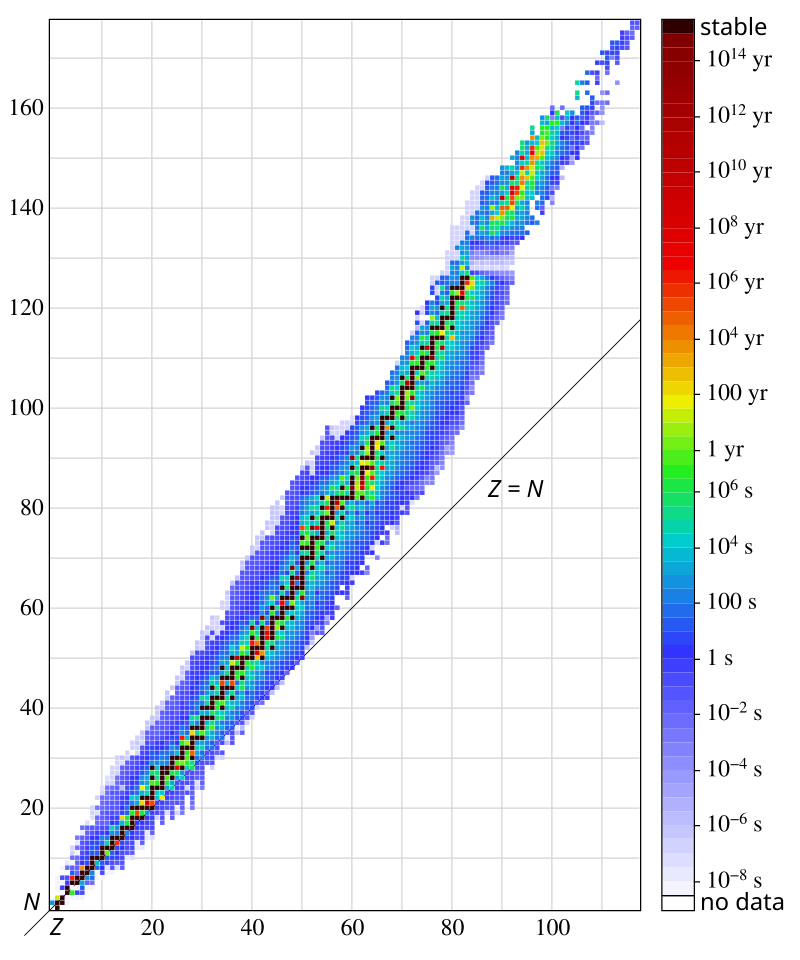
\includegraphics[width = 0.75\textwidth]{segre-chart.png}
  \caption{Tavola di Segré.}
  \label{segre-chart}
\end{figure}
\begin{figure}
  \centering
  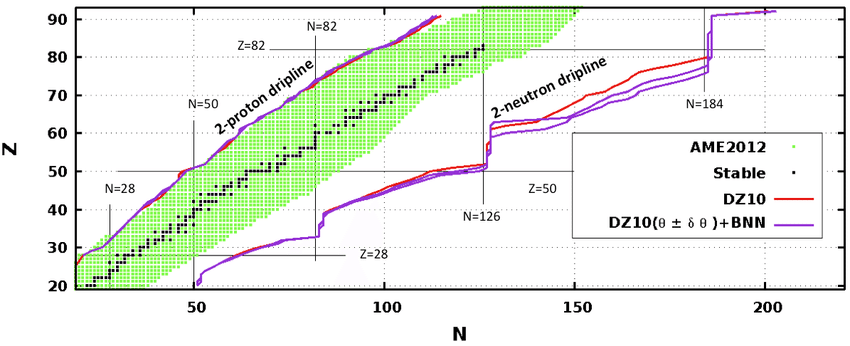
\includegraphics[width = 0.55\textwidth]{drip-lines.png}
  \caption{Nuclear driplines.}
  \label{drip-lines}
\end{figure}

\section{Evidenze sperimentali}

Le prime evidenze sperimentali dell'esistenza del nucleo atomico si devono al gruppo di ricerca di Rutherford, Geiger e Marsden: prima di loro, Thomson era riuscito ad estrarre delle cariche negative dall'atomo, identificando l'elettrone, ed aveva di conseguenza formulato la sua teoria della struttura atomica come sfera carica positivamente in cui sono immersi gli elettroni ($ \virgolette{plum pudding} $ model).\\
Con i loro esperimenti, Rutherford et al. dimostrarono invece che le cariche positive erano concentrate in una regione piccola al centro dell'atomo.

\subsection{Scattering di Rutherford}

L'esperimento condotto da Rutherford et al. consiste nell'irradiare una lamina sottile di oro con un fascio di particelle $ \alpha $ (nuclei di $ \ch{^{4} He} $): a livello puramente cinematico (ignorando la natura dell'interazione tra beam e target), essendo la velocità delle particelle $ \alpha $ $ v_0 \sim 0.1c $, è possibile trattare il problema come un urto elastico non-relativistico:
\begin{equation}
	\begin{cases}
	  m_{\alpha} \ve{v}_0 = m_{\alpha} \ve{v}_f + m_t \ve{v}_t \\
	  m_{\alpha} v_0^2 = m_{\alpha} v_f^2 + m_t v_t^2 \\
	\end{cases}
	\label{eq:2}
\end{equation}
Combinando le due equazioni e definendo $ \theta $ l'angolo tra $ \ve{v}_f $ e $ \ve{v}_t $:
\begin{equation}
	\cos \theta = \frac{1}{2} \frac{v_t}{v_f} \left(1 - \frac{m_t}{m_{\alpha}}\right)
	\label{eq:3}
\end{equation}
Si possono distinguere due principali casi:
\begin{enumerate}
	\item $ m_t \ll m_{\alpha} $: $ \cos \theta > 0 $, dunque si parla di forward scattering, poiché non sono possibili grossi valori di $ \theta $;
	\item $ m_t \gg m_{\alpha} $: $ \cos \theta < 0 $, dunque diventano possibili anche angoli prossimi $ \pi $.
\end{enumerate}
Il modello di Thomson rientra nella prima casistica, poiché in tal caso all'interno dell'atomo lo scattering può avvenire solo con gli elettroni, che hanno $ m_e \ll m_{\alpha} \approx 4m_p $.\\
Ciò che Rutherford et al. osservarono, però, è che occasionalmente delle particelle $ \alpha $ vengono riflesse dalla lamina d'oro: questo risultato è incompatibile con lo scattering con elettroni o con una carica positiva diffusa, dunque fu confermato che la carica positiva nell'atomo è concentrata in un unico punto massivo, il nucleo atomico.

\subsubsection{Rutherford cross-section}

Nella trattazione cinematica è stata ignorata l'interazione tra particelle $ \alpha $ e nucleo atomico, che è ciò che effettivamente determina lo scattering: essa può essere modellata, in forma approssimativa (in particolare per parametro d'urto compreso tra il raggio nucleare e l'orbita elettronica più interna), dal potenziale coulombiano; dette $ Z $ il numero atomico dell'atomo target e $ Z' $ quello degli atomi del beam (nel caso specifico dello scattering di Rutherford $ Z = Z_{\ch{Au}} = 79 $ e $ Z' = Z_{\ch{He}} = 4 $), il potenziale d'interazione è:
\begin{equation}
	V(\ve{r}) = \frac{ZZ' e^2}{r}
	\label{eq:4}
\end{equation}
Dalla meccanica classica è possibile legare il parametro d'urto $ b $ all'angolo di scattering $ \theta $:
\begin{equation}
	b = \frac{ZZ' e^2}{2 E_0} \cot \frac{\theta}{2}
	\label{eq:5}
\end{equation}
dove $ E_0 $ è l'energia della particella incidente.\\
È anche possibile ricavare una stima del raggio nucleare: esso può essere approssimato dalla distanza di closest-approach $ a $, ovverosia il valore per cui vale la condizione $ E_0 = V(a) $.\\
Per calcolare la cross-section dello scattering di Rutherford, si consideri un fascio incidente monoenergetico con energia $ E_0 $ e $ N_0 $ particelle incidenti per unità di area e di tempo: facendo variare il parametro d'urto tra $ b $ e $ b + db $, dunque variando l'angolo di scattering tra $ \theta $ e $ \theta - d \theta $, si avranno $ 2\pi N_0 b \,db $ particelle incidenti per unità di tempo (data la sezione d'urto $ \Delta\sigma = 2\pi b \,db $, Fig. \ref{rutherford}).
\begin{figure}
	\centering
	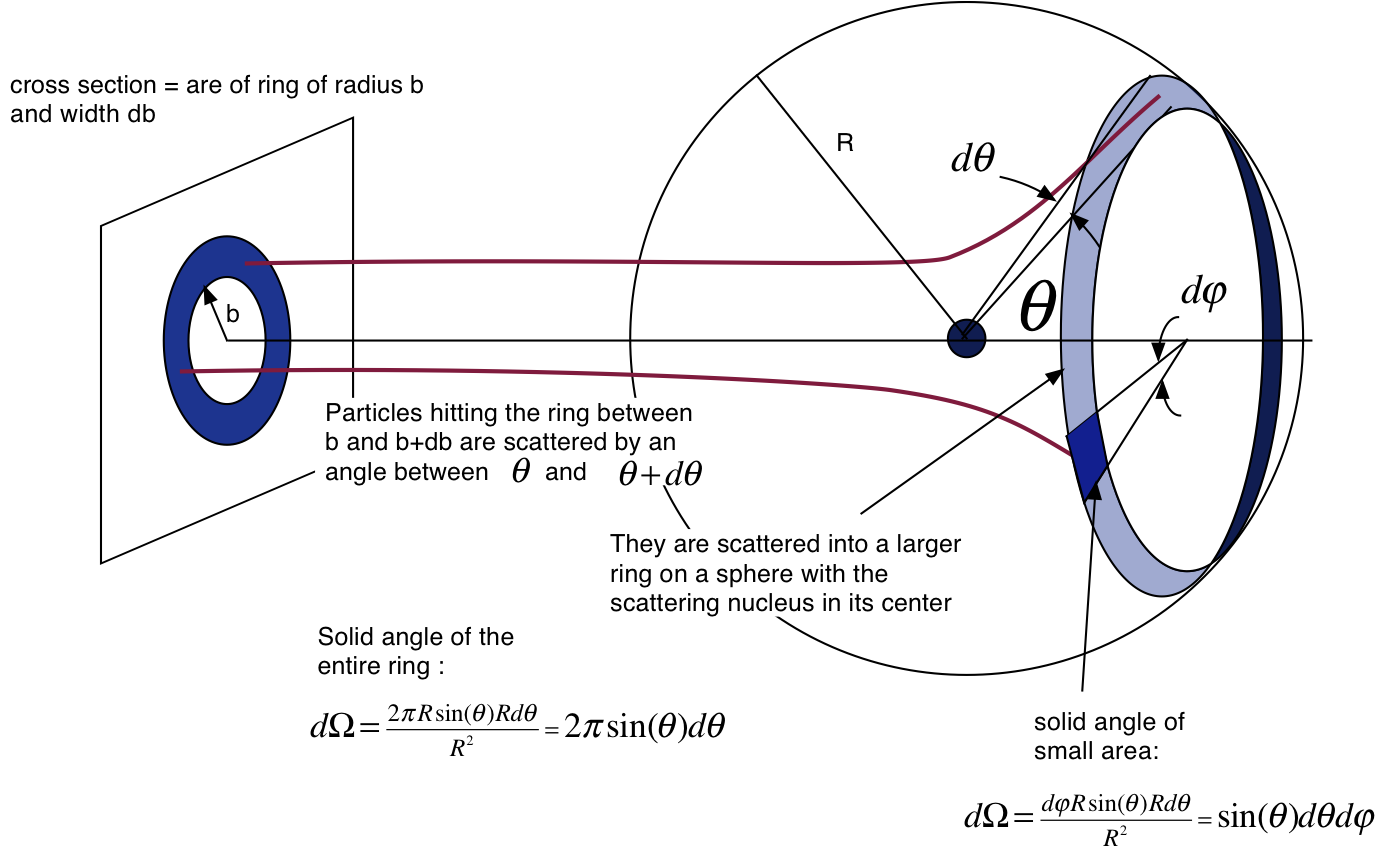
\includegraphics[width=0.95\textwidth]{rutherford.png}
	\caption{Sezione d'urto dello scattering di Rutherford.}
	\label{rutherford}
\end{figure}

Va notato che è possibile ignorare il fatto che la lamina target ha un numero elevato di atomi target e che ogni partiella nel beam incidente ha un diverso parametro d'urto relativo a ciascuno di essi, poiché la lastra è considerata così sottile da rendere improbabili collisioni multiple della stessa particella incidente; inoltre, dal modello atomico di Rutherford ricaviamo che i nuclei atomici si trovano a distanze grandi rispetto alle loro dimensioni, rendendo significative solo le traiettorie con parametro d'urto vicino al nucleo atomico.\\
Nel caso di un potenziale d'interazione generico, $ \Delta\sigma $ può avere anche dipendenza azimuthale:
\begin{equation}
	\Delta\sigma(\theta,\phi) = b \,db\,d\phi = - \frac{d\sigma}{d\Omega} (\theta,\phi) \,d\Omega= - \frac{d\sigma}{d\Omega} (\theta,\phi) \sin \theta \,d\theta\,d\phi
	\label{eq:6}
\end{equation}
dov'è stata utilizzata la differential cross-section $ \frac{d\sigma}{d\Omega} $ e dove si è tenuto conto che un aumento di $ b $ porta ad una diminuzione di $ \theta $ tramite il segno negativo.\\
Essendo il potenziale coulombiano un potenziale centrale a simmetria sferica, è possibile semplificare il calcolo grazie alla simmetria azimuthale, ottenendo:
\begin{equation}
	\frac{d\sigma}{d\Omega} (\theta) = - \frac{b}{\sin \theta} \frac{db}{d\theta}
	\label{eq:7}
\end{equation}
Lo scattering di Rutherford può essere quindi completamente caratterizzato utilizzando l'Eq. \ref{eq:5}:
\begin{equation}
	\frac{d\sigma}{d\Omega} (\theta) = \left( \frac{ZZ' e^2}{4 E_0} \right)^2 \frac{1}{\sin^2 \frac{\theta}{2}}
	\label{eq:8}
\end{equation}
È anche possibile definire la sezione d'urto totale $ \sigma_{\text{tot}} $ come:
\begin{equation}
	\sigma_{\text{tot}} = \int_{\Omega} \frac{d\sigma}{d\Omega} (\theta,\phi) \,d\Omega
	\label{eq:9}
\end{equation}
Essa rappresenta una sorta di area di scattering effettiva che la sorgente del potenziale determina a tutti i possibili valori del parametro d'urto.\\
Nel caso dello scattering di Rutherford:
\begin{equation}
	\begin{split}
		\sigma_{\text{tot}} &= \int_0^{2\pi} \int_0^{\pi} \frac{d\sigma}{d\Omega} (\theta,\phi) \sin \theta \,d\theta\,d\phi = 2\pi \int_0^{\pi} \frac{d\sigma}{d\Omega} (\theta) \sin \theta \,d\theta \\
				    &= 8\pi \left( \frac{ZZ' e^2}{4 E_0} \right)^2 \int_0^1 \frac{1}{\sin^3 \frac{\theta}{2}} d\left( \sin \frac{\theta}{2} \right) \longrightarrow \infty
	\end{split}
	\label{eq:10}
\end{equation}
Questo risultato divergente è coerente con l'interpretazione data della sezione d'urto totale: il potenziale coulombiano è associato all'interazione elettromagnetica, la quale ha un range infinito, dunque anche l'area efficace di scattering sarà infita.\\
In maniera realistica, però, si può considerare che dopo un determinato valore di cutoff $ b_0 $ lo scattering non abbia più effetti osservabili sulla particella incidente, dunque la sezione d'urto totale osservabile si ottiene integrando la differential cross-section tra $ 0 $ e $ \theta_0 < \pi$, ottenendo dunque un valore finito.

\subsection{Scattering elettronico}

Data la dualità onda-particella che risulta da una descrizione quanto-meccanica della materia, la sezione d'urto da scattering non sarà determinata soltanto dall'interazione coulombiana ma anche da effetti diffrattivi, evidenziati dal pattern di diffrazione in Fig. \ref{diffraction}: l'analogo ottico è la diffrazione da disco opaco, poiché il nucleo atomico assorbe nucleoni, con la dovuta differenza che la superficie del nucleo ha una determinata diffusività, la quale determina dei minimi non-nulli nello spettro di diffrazione.
\begin{figure}
	\centering
	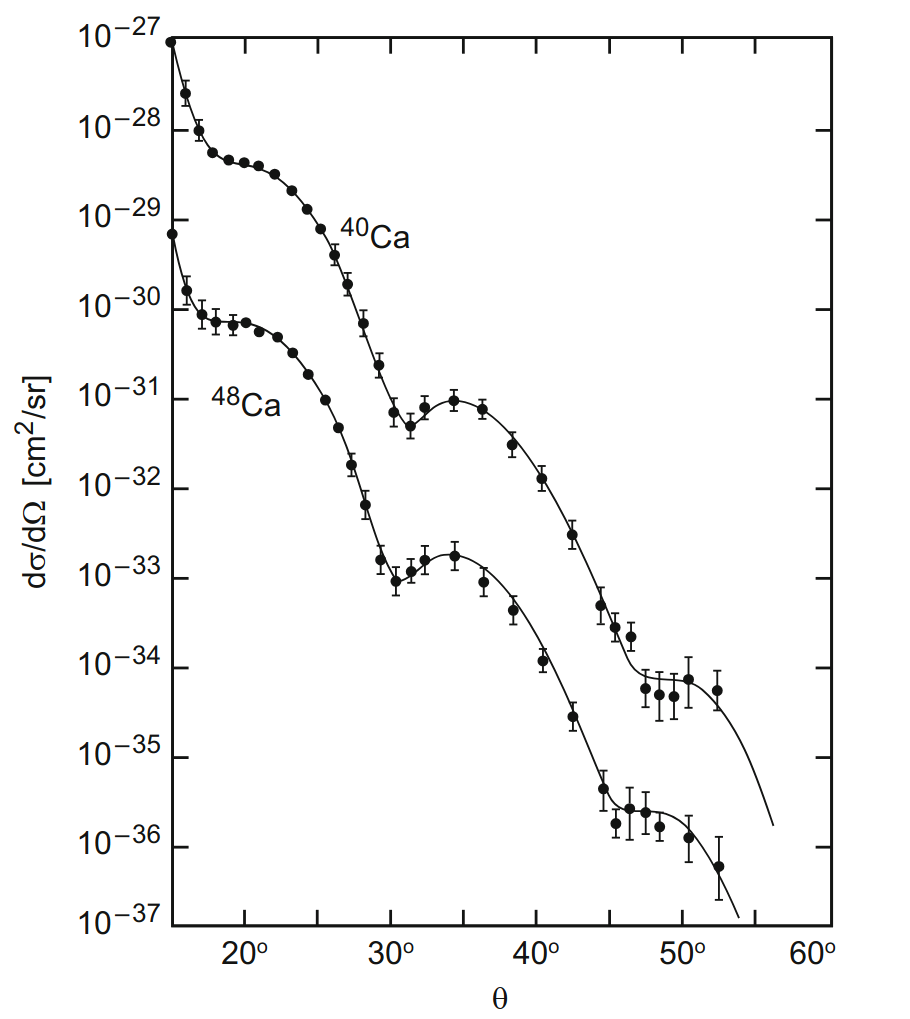
\includegraphics[width=0.95\textwidth]{diffraction.png}
	\caption{Sezione d'urto dello scattering elettronico.}
	\label{diffraction}
\end{figure}
Per evitare che all'interazione coulombiana si sovrapponga anche quella tra nucleoni, per studiare la struttura del nucleo atomico le sonde migliori sono gli elettroni: poiché per sondare una scala di lunghezze $ \Delta x $ è necessaria una lunghezza d'onda $ \lambda \sim \Delta x $, dalla relazione di de Broglie si ha che la quantità di moto degli elettroni incidenti deve essere $ p \sim h / \Delta x $. La struttura del nucleo atomico risulta visibile su scale di $ 1\fm $, dunque sono necessari elettroni con momento lineare $ p \approx 200 \mev/c $; nel caso si voglia studiare la struttura interna dei nucleoni, la stima aumenta di almeno un ordine di grandezza.\\
Ricordando che $ E^2 = p^2 c^2 + m_0^2 c^4 $ ed $ E = K + m_0 c^2 $, considerando che $ m_e = 0.511 \mev/c^2 $, si vede che gli elettroni utilizzati per sondare il nucleo atomico sono in regime ultra-relativistico, duqnue nel calcolo della cross-section sono da tenere in conto effetti relativistici legati allo spin ed il nuclear recoil: trascurando quest'ultimo, si può applicare una correzione alla Rutherford cross-section, detta Mott cross-section:
\begin{equation}
	\left(\frac{d\sigma}{d\Omega}\right)_{\text{Mott}} = \left(\frac{d\sigma}{d\Omega}\right)_{\text{Ruth}} \left(1 - \beta^2 \sin^2 \frac{\theta}{2}\right)
	\label{eq:11}
\end{equation}
Queste sezioni d'urto, però, considerano scattering tra oggetti puntiformi, ma mentre un elettrone può effettivamente essere considerato tale a queste scale di lunghezza, lo stesso non si può dire per il nucleo atomico, il quale avrà una certa distribuzione di carica $ \rho(\ve{r}) $ estesa nello spazio; per considerare anche questo fatto, nel calcolo della cross-section si applica un'ulteriore correzione:
\begin{equation}
	\frac{d\sigma}{d\Omega} = \left(\frac{d\sigma}{d\Omega}\right)_{\text{Mott}} \abs{F(q)}^2
	\label{eq:12}
\end{equation}
dove $ \abs{F(q)}^2 $ è detto form factor e $ \ve{q} \defeq \frac{1}{\hbar} \abs{\ve{p}' - \ve{p}} $, con $ \ve{p} $ e $ \ve{p}' $ momento iniziale e finale dell'elettrone. Dato che si sta considerando uno scattering elastico, si ha $ p = p' $ e dunque $ q = \frac{1}{\hbar} 2p \sin \frac{\theta}{2} $, con $ \theta $ angolo di scattering.\\
Nel caso dell'approssimazione di Born (elettroni come onde piane $ \psi(\ve{r}) = \frac{1}{\sqrt{V}} e^{i \ve{p}\cdot\ve{x} / \hbar} $) e trascurando il nuclear recoil, il form factor è la trasformata di Fourier della distribuzione di carica $ \rho(\ve{r}) $:
\begin{equation}
	F(q) = \int_{r \le R} e^{i \ve{p}\cdot\ve{r} / \hbar} \rho(\ve{r}) d^3\ve{r}
	\label{eq:13}
\end{equation}
con $ R $ raggio nucleare ed opportuna normalizzazione $ F(0) = 1 $.\\
In questa approssimazione, quindi, una misura della cross-section di scattering elettronico può dare informazioni sulla distribuzione di carica nel nucleo atomico; inoltre, è possibile dare una stima del raggio nucleare dallo studio dello spettro di diffrazione evidenziato dalla cross-section, poiché il primo minimo di diffrazione è dato da $ \frac{q}{\hbar} \approx \frac{4.5}{R} $; se invece si considerano due isotopi, dal fatto che la separazione angolare tra due minimi è data $ \Delta\theta = \frac{\hbar}{p R} $ si evince che all'aumentare del numero di massa aumenta anche il raggio atomico (vedere Fig. \ref{diffraction}).

\subsubsection{Distribuzione di carica nucleare}

Compiendo esperimenti di scattering elettronico e raccogliendo dati relativi a vari nuclei atomici, si è giunti alla conclusione che i nuclidi non sono sfere con un confine ben delineato, ma al loro interno la densità di carica si mantiene approssimativamente costante, mentre verso la superficie essa si riduce su un intervallo radiale relativamente ampio; la distribuzione di carica nucleare può dunque essere approssimata da una distribuzione di Fermi:
\begin{equation}
	\rho(\ve{r}) = \frac{\rho_0}{1 + e^{(r - c) / a}}
	\label{eq:14}
\end{equation}
dove i parametri empirici valgono (per nuclei pesanti) $ c = 1.07\fm \cdot A^{1/3} $ e $ a = 0.54\fm $.\\
Una volta nota la distribuzione di carica, è possibile calcolare il raggio quadratico medio: per nuclei medi e pesanti, si ha $ \sqrt{\langle r^2 \rangle} = r_0 A^{1/3} $, con $ r_0 = 0.94\fm $. Se si approssima il nucleo come una sfera uniformemente carica, il suo raggio, definito come raggio nucleare, è dato da $ R^2 = \frac{5}{3} \langle r^2 \rangle $, ovvero $ R = R_0 A^{1/3} $, con $ R_0 = 1.21\fm $ (questa è la definizione più diffusa di raggio nucleare).\\
È anche possibile definire una skin depth (o surface thickness) $ t $ come lo spessore del guscio sferico in cui la densità di carica diminuisce dal $ 90\% $ al $ 10\% $ del suo valore massimo: per nuclei pesanti, si trova $ t = 2a\ln9 \approx 4.4 a $.\\
Come si può vedere in Fig. \ref{charge-distr}, la densità di carica centrale $ \rho_0 $ diminuisce leggermente all'aumentare del numero di massa; se però viene considerata la presenza di neutroni e si moltiplica per un fattore $ A / Z $, si trova un valore quasi identico per tutti i nuclidi (questo è coerente con $ R \sim A^{1/3} $, poiché così $ \rho_0 \sim A / V $ rimane costante): questo corrisponde alla densità che teoricamente avrebbe della materia nucleare infinitamente estesa, pari a $ \rho_n \approx 0.17 \,\text{nucleoni} / \text{fm}^3 $, che corrisponde a $ c = 1.12\fm \cdot A^{1/3} $.\\
Sperimentalmente si trova che alcuni nuclidi (ad esempio i lantanidi) non hanno una forma sferica ma assumono deformazioni ellissoidali: queste forme non possono essere studiate con scattering elettronico, poiché esso evidenzia soltanto una superficie molto diffusa.\\
Va infine notato che nuclidi leggeri come $ \ch{^{6,7}Li} $, $ \ch{^{9}Be} $ e soprattutto $ \ch{^{4}He} $ costituiscono dei casi speciali: essi non presentano una densità di carica centrale costante, ma il suo andamento è approssimativamente gaussiano.
\begin{figure}
	\centering
	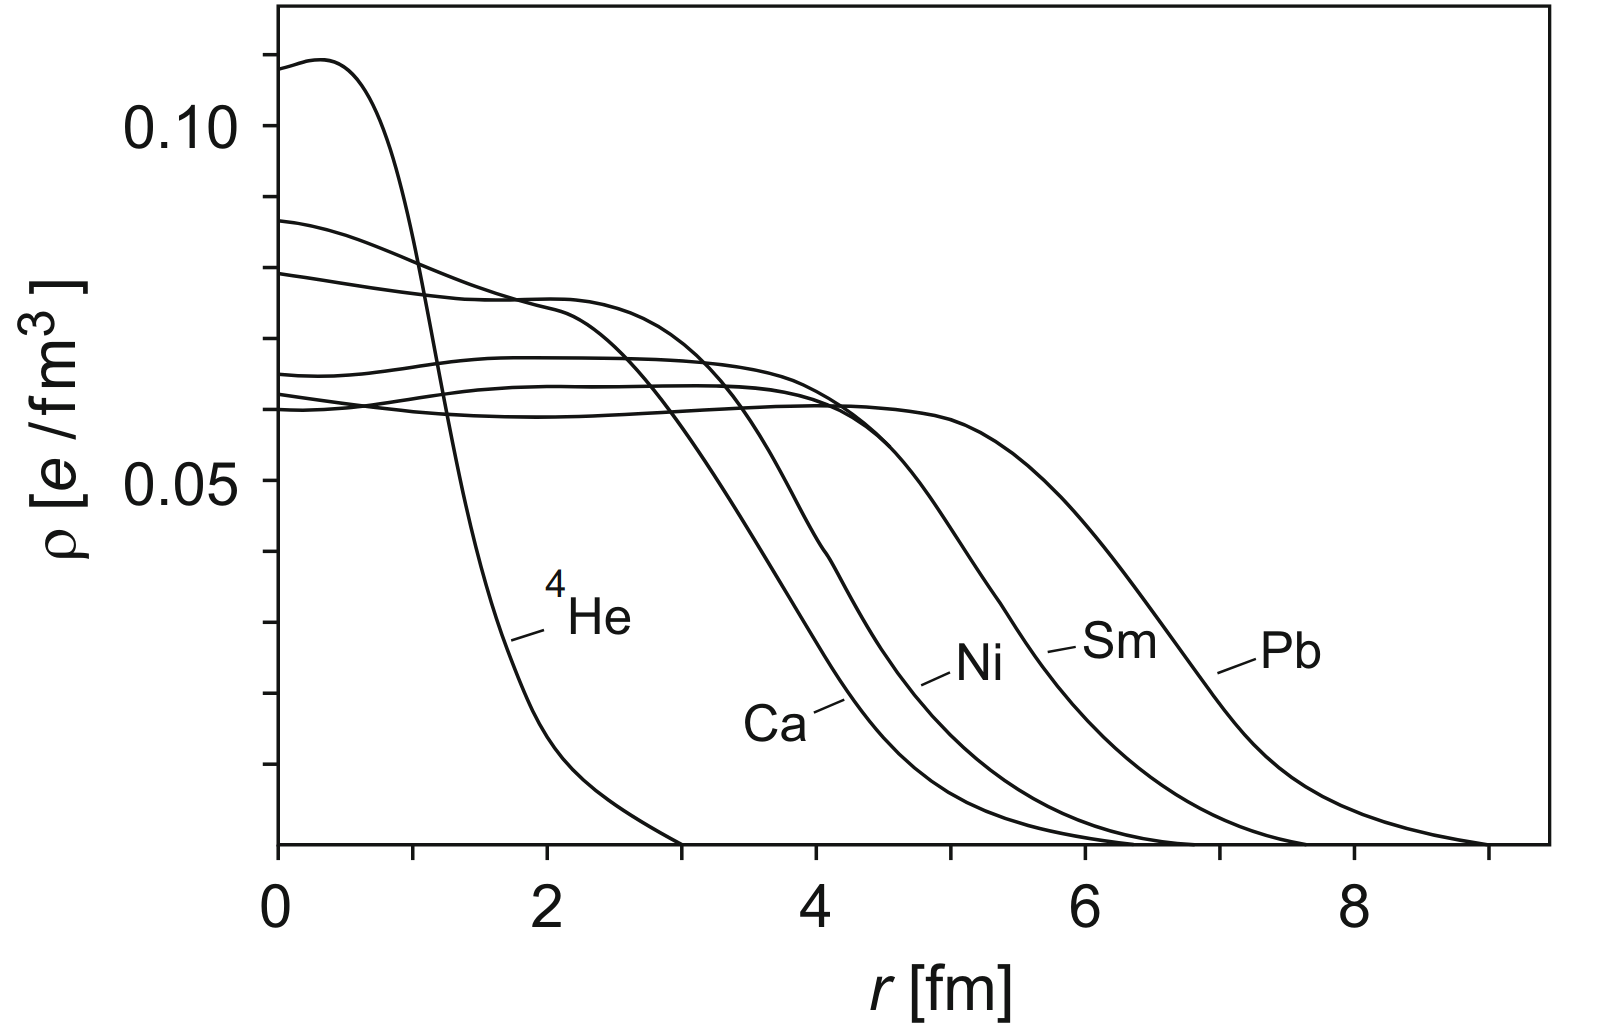
\includegraphics[width=0.75\textwidth]{charge-distribution.png}
	\caption{Distribuzione di carica in vari nuclidi.}
	\label{charge-distr}
\end{figure}


\subsubsection{Luminosità}

Nello studio dei rilevatori di scattering un importante parametro è la luminosità:
\begin{equation}
	\mathcal{L} = N_b N_t
	\label{eq:15}
\end{equation}
dove $ N_b $ è il numero di particelle incidenti per unità di tempo e $ N_t $ il numero di nuclidi target per unità d'area.\\
Questo parametro è legato all'efficienza del rilevatore, misurata dal numero di eventi rilevati nell'unità di tempo $ \dot{N} $:
\begin{equation}
	\dot{N} (E, \theta) = \mathcal{L}\, \frac{d\sigma}{d\Omega} (E,\theta) \,\Delta\Omega
	\label{eq:16}
\end{equation}
Nel caso dello scattering elettronico, la cross-section è molto piccola, dunque sono necessari collisori dall'elevata luminosità (tecnicamente difficile): si va da $ \mathcal{L} \sim 10^{26} \,\text{cm}^2 / s $ per sondare nuclidi con $ Z \sim 80 $ a $ \mathcal{L} \sim 10^{31} \,\text{cm}^2 / s $ per $ Z \sim 10 $.










